\documentclass[dvipdfmx]{jsarticle}
\usepackage[T1]{fontenc}
\usepackage[dvipdfmx]{hyperref}
\usepackage{lmodern}
\usepackage{latexsym}
\usepackage{amsfonts}
\usepackage{amssymb}
\usepackage{mathtools}
\usepackage{amsthm}
\usepackage{multirow}
\usepackage[dvipdfmx]{graphicx}
\usepackage{wrapfig}
\usepackage{here}
\usepackage{float}
\usepackage{ascmac}
\usepackage{url}

\title{人物相関図の可視化-課題研究3-}
\author{文理学部情報科学科\\5419045 高林 秀}
\date{\today}

\begin{document}

\maketitle

\begin{abstract}
本稿は、今年度コンピューティング2のネットワークの可視化に関する課題として、小説レ・ミゼラブルの人物相関図をグラフで可視化する実験を行うものである。なお、本課題ではp5.jsを使用した。
\end{abstract}

\section{目的}
本稿は、今年度コンピューティング2の課題研究として「ネットワークの可視化」に関する問題に解答するものである。また同時に、問題に関する計算理論についても復習するものとする。
\section{計算理論}
今回の実験で使用したForce-directedアルゴリズムについて、関連する用語もセットで説明する。
\subsection{グラフ描画について}
数学的なグラフ理論におけるグラフは、ノードの集合とノード間を結ぶ辺、すなわちリンクより成立している。グラフはノード間のつながりという関係のみを持つが、グラフの構造までは2,3次元に描画してみないと視覚化することができない。画面にノードとリンクを直接的に描画した図をノードリンク図と呼ぶ。\par
ノードリンク図を描画するにあたって、ノードを画面上のどの位置に描画させるか決定しなければならない。すなわち、グラフの描画とはノードの画面上での位置を決定する操作を指す。\par
一般に、グラフのどの特徴を描画するかによってグラフ描画の手法は異なってくる。グラフ描画によって可視化されるグラフ構造は様々なネットワークや、データ構造の理解に役立てることが可能である。
\begin{figure}[H]
  \centering
  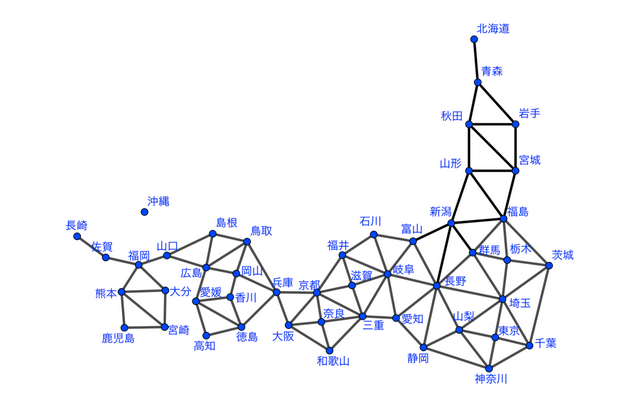
\includegraphics[scale=0.6]{images/graph_img.png}
  \caption{グラフ描画の例}
  出典:\url{https://qiita.com/drken/items/4a7869c5e304883f539b}
\end{figure}

\subsection{Force-directedアルゴリズム}
グラフ描画の手法の1つとして、Force-directedアルゴリズムが存在する。このアルゴリズムは、ノード間に作用する力をシミュレーションすることによりノードの座標を決定する。ノード間のリンクをバネと見なして、その運動をシミュレーションし描画する。このように、リンクをバネと見なしてグラフ描画を行うことをバネモデルと呼ぶ。バネモデルの有名なグラフ描画として、Eadasの方法が挙げられる。Eadasの方法に関して本稿では、詳細な説明は扱わないが、下記のリンクを参照いただきたい。
\begin{itemize}
  \item Eadasの方法:\url{http://www2.kobe-u.ac.jp/~ky/labo/research/graph-drawing.htm}
\end{itemize}
本稿では、後述するVerlet法により実現できるバネモデルの描画を行う。
下記のコードはForce-directedアルゴリズムによって可視化したノード数10個のグラフを描画したものである。各ノードのペアは$\frac{1}{2}$の確率でリンクを持つようにランダムにグラフを生成している。
\begin{verbatim}
  let n;
  let x;
  let y;
  let vx;
  let vy;

  let m;
  let source;
  let target;

  const r = 25;

  function setup() {
    createCanvas(600, 600);
    initializeGraph(10);
    for (let i = 0; i < n; ++i) {
      x[i] = random(width);
      y[i] = random(height);
    }
    vx.fill(0);
    vy.fill(0);
  }

  function draw() {
    drawObjects();
    updatePosition();
    updateVelocity();
  }

  function initializeGraph(k) {
    n = k;
    x =  new Array(n);
    y =  new Array(n);
    vx = new Array(n);
    vy = new Array(n);
    m = 0;
    source = new Array();
    target = new Array();
    for (let i = 0; i < n; ++i) {
      for (let j = i + 1; j < n; ++j) {
        if (random(1) < 0.5) {
          source.push(i);
          target.push(j);
          m += 1;
        }
      }
    }
  }

  function drawObjects() {
    background(255);
    for (let i = 0; i < m; ++i) {
      const s = source[i];
      const t = target[i];
      line(x[s], y[s], x[t], y[t]);
    }
    for (let i = 0; i < n; ++i) {
      fill(255);
      ellipse(x[i], y[i], 2 * r, 2 * r);
      fill(0);
      textSize(32);
      textAlign(CENTER, CENTER);
      text(i, x[i], y[i]);
    }
  }

  function updatePosition() {
    for (let i = 0; i < n; ++i) {
      x[i] += vx[i];
      y[i] += vy[i];
    }
  }

  function updateVelocity() {
    applySpringForce(0.001, 10);
    applyRepulsiveForce(10);
    applyResistanceForce(0.01);
    applyCentering();
  }

  function applySpringForce(k, L) {
    for (let i = 0; i < m; ++i) {
      const s = source[i];
      const t = target[i];
      const d = dist(x[s], y[s], x[t], y[t]);
      const theta = atan2(y[s] - y[t], x[s] - x[t]);
      const w = k * (L - d);
      vx[s] += w * cos(theta);
      vy[s] += w * sin(theta);
      vx[t] -= w * cos(theta);
      vy[t] -= w * sin(theta);
    }
  }

  function applyRepulsiveForce(q) {
    for (let i = 0; i < n; ++i) {
      for (let j = 0; j < n; ++j) {
        if (i === j) {
          continue;
        }
        const d = distance(i, j);
        const w = -q / (d * d);
        vx[i] += (x[j] - x[i]) * w;
        vy[i] += (y[j] - y[i]) * w;
      }
    }
  }

  function applyResistanceForce(k) {
    for (let i = 0; i < n; ++i) {
      vx[i] += -k * vx[i];
      vy[i] += -k * vy[i];
    }
  }

  function applyCentering() {
    let cx = 0;
    let cy = 0;
    for (let i = 0; i < n; ++i) {
      cx += x[i];
      cy += y[i];
    }
    cx /= n;
    cy /= n;
    for (let i = 0; i < n; ++i) {
      x[i] += -cx + width / 2;
      y[i] += -cy + height / 2;
    }
  }

  function distance(i, j) {
    const minDistance = 10;
    const d = dist(x[i], y[i], x[j], y[j]);
    if (d < minDistance) {
      return minDistance;
    }
    return d;
  }
\end{verbatim}

\end{document}
